% ****** Start of file apssamp.tex ******
%
%   This file is part of the APS files in the REVTeX 4.2 distribution.
%   Version 4.2a of REVTeX, December 2014
%
%   Copyright (c) 2014 The American Physical Society.
%
%   See the REVTeX 4 README file for restrictions and more information.
%
% TeX'ing this file requires that you have AMS-LaTeX 2.0 installed
% as well as the rest of the prerequisites for REVTeX 4.2
%
% See the REVTeX 4 README file
% It also requires running BibTeX. The commands are as follows:
%
%  1)  latex apssamp.tex
%  2)  bibtex apssamp
%  3)  latex apssamp.tex
%  4)  latex apssamp.tex
%
\documentclass[%
 reprint,
%superscriptaddress,
%groupedaddress,
%unsortedaddress,
%runinaddress,
%frontmatterverbose, 
%preprint,
%preprintnumbers,
%nofootinbib,
%nobibnotes,
%bibnotes,
 amsmath,amssymb,
 aps,
%pra,
%prb,
%rmp,
%prstab,
%prstper,
%floatfix,
]{revtex4-2}

\usepackage{graphicx}% Include figure files
\usepackage{dcolumn}% Align table columns on decimal point
\usepackage{bm}% bold math
\usepackage{chemformula}
\usepackage{booktabs} 
\usepackage{float} 
\begin{document}

\preprint{APS/123-QED}

\title{Calculating Crystal Field Splitting \\ via Wannier Functions}% Force line breaks with \\
\thanks{A footnote to the article title}%

\author{Valentina Mazzotti}
 \altaffiliation[Also at ]{McGill University}
 \email{Second.Author@institution.edu}
\affiliation{%
 Department of Physics, McGill University, Montreal, Quebec H3A 2T8, Canada \\
}
\date{\today}% It is always \today, today,
             %  but any date may be explicitly specified

\begin{abstract}

This study presents a method for calculating the crystal field splitting \(\Delta_{\text{o}}\) utilizing Maximally Localized Wannier Functions (MLWF) in two cubic perovskites, \ch{SrVO_3} and \ch{TiPbO_3}.  First, high-quality Wannier functions are constructed, which are then used to derive the crystal field splitting for these materials. By constructing tailored sets of Wannier functions with varying levels of hybridization, we demonstrate this approach using \ch{SrVO_3} as a representative transition metal oxide, where the \(t_{2g}\) and \(e_{g}\) states are clearly separated.  Subsequently, we apply the same technique to the cubic perovskites \ch{TiPbO3}, which displays a band structure with overlapping groups of bands,  lacking the distinct separation between different dominant orbital characters seen in \ch{SrVO_3}.
 By constructing tailored sets of Wannier functions with varying levels of hybridization, we analyze trends in crystal field splitting and showcase how hybridization with the surrounding ligand \(p\) and \(s\)-orbitals contributes significantly to the ligand field splitting. Lastly, we compare the calculated crystal field splitting obtained via MLWFs and the predictions from a simple classical point charge model. 

\end{abstract}

%\keywords{Suggested keywords}%Use showkeys class option if keyword
                              %display desired
\maketitle
\section{Introduction}
One of the foundational concepts in the theory of transition metal (TM) oxides is the interaction of a TM ion with the electrostatic potential created by its surrounding ions, known as the crystal field \cite{griffith1961theory}. Crystal field theory predicts that in transition metal oxides, particularly in perovskites, the \(d\)-orbitals of the TM cation split into two energy levels: the lower-energy \(t_{2g}\) orbitals and the higher-energy \(e_g\) orbitals, separated by the crystal field splitting energy. This splitting results from the interaction between the \(d\)-electrons of the TM ion and the electrostatic field generated by surrounding anions, influencing phenomena such as magnetism, Mott insulating behavior, and Jahn-Teller distortions \cite{CFT_Theory}.
For the past 30 years, density functional theory (DFT) has been the dominant method for the quantum mechanical simulation of periodic systems, as it provides a computationally efficient approach for studying the electronic structure of atoms, molecules, and solids \cite{DFT}. While the electronic ground state of a periodic system is often described using extended Bloch orbitals, an alternative representation in terms of localized "Wannier functions" was introduced by Gregory Wannier in 1937 \cite{Marzari2012}. By combining DFT with maximally localized Wannier functions (MLWFs) \cite{Marzari1997}, we can calculate the on-site energies of \(d\)-orbitals and determine the crystal field splitting in transition metal oxides \cite{Scaramucci2014}. In this study, we apply this approach to two perovskites, \ch{SrVO_3} and \ch{TiPbO_3}, reconstructing the electronic structure to extract crystal field splitting values. 
In this work, we investigate the crystal field splitting in the perovskites \ch{SrVO_3} and \ch{TiPbO_3} by reconstructing their electronic structures using density functional theory (DFT) combined with maximally localized Wannier functions (MLWFs). By constructing sets of Wannier functions corresponding to different energy windows, we successively isolate the effects of hybridization with various ligand states and identify the hybridization component in the derived crystal field splitting.
The paper is organized as follows: I will present the theory of CFT and the construction of MLWF in the Theory section, then I will briefly present the workflow that I used to construct a simplified yet accurate description of the electronic structure, allowing me to derive the crystal field splitting.  We then present results for two perovskite oxide, where we evaluate the effect of
\subsection{Crystal field splitting in octahedral complexes}
Crystal field theory (CFT) describes the breaking of degeneracies of electron orbital states, usually $d$ or $f$ orbitals, due to a static electric field produced by a surrounding charge distribution (the anion neighbors) \cite{bethe1929termaufspaltung}. As a ligand approaches the metal ion, the electrons from the ligand will be closer to some of the d-orbitals and farther away from others, causing a loss of degeneracy, and giving rise to the characteristic energy splitting of the d-orbitals. This split is influenced by factors such as the metal's  oxidation state, ligand geometry and arrangement, the coordination number, and the type of ligands \cite{penney1932influence}, which means that each system has its own crystal field splitting, and precise derivations of its value can only be found either by experiment or by \textit{ab-initio} calculations on the system itself. 
The most common type of complex investigated in CFT is octahedral, in which six ligands form the vertices of an octahedron around the metal ion. 
Taking \ch{SrVO_3} as an example, we can illustrate the crystal field splitting of the \(d\)-orbitals in an octahedral complex. In SrVO\(_3\), the vanadium (V) atom, shown in light blue in Fig. \ref{fig:SrVO3_structure}, is positioned at the center of an octahedron formed by six surrounding oxygen (O) atoms (red). This octahedral arrangement of ligands (O\(^{2-}\) anions) creates a crystal field that interacts with the \(d\)-orbitals of the central V\(^{4+}\) ion, which has a \(3d^1\) electron configuration. In octahedral symmetry, the \(d\)-orbitals split into two sets with an energy difference, \(\Delta_{\text{oct}}\) \cite{InfluenceOfCrystallineFields, CFT_Theory}. In this environment, the \(d_{xy}\), \(d_{xz}\), and \(d_{yz}\) orbitals experience less repulsion from the ligands and are therefore lower in energy, collectively referred to as the \(t_{2g}\) set. In contrast, the \(d_{z^2}\) and \(d_{x^2-y^2}\) orbitals, which are oriented directly towards the ligands, experience higher repulsion and form the higher-energy \(e_g\) set. 
\begin{figure}[htb]
    \centering
    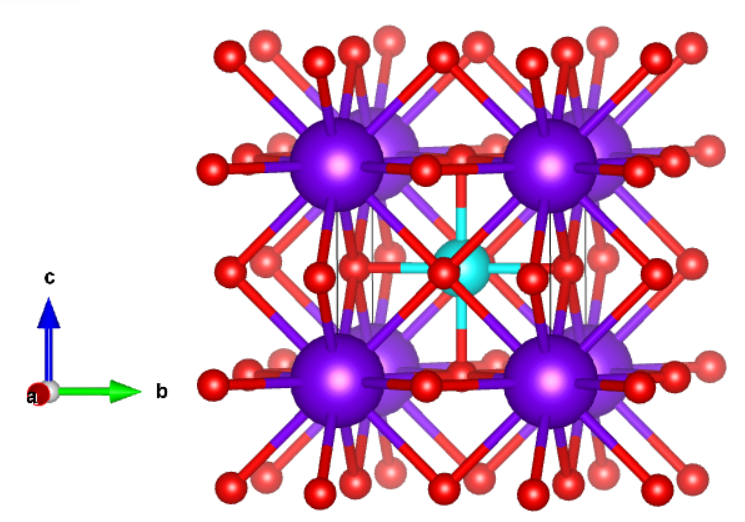
\includegraphics[width=\linewidth]{figs/SrVO3_poscar.PNG}
    \caption{\ch{SrVO_3} serves as a prototypical example of a transition metal oxide, where the \(3d\) orbitals of V\(^{4+}\) ions experience crystal field splitting due to the surrounding oxygen ligands, resulting in a characteristic separation between the \(t_{2g}\) and \(e_g\) orbitals \cite{Scaramucci2014}.}
    \label{fig:SrVO3_structure}
\end{figure}


\subsection{Construction of Maximally Localized Wannier Functions}
The electronic states within a solid are typically represented by Bloch states, which correspond to the eigenfunctions of the single-particle Hamiltonian for electrons in the periodic effective crystal potential. Since in this work we are employing density functional theory (DFT), the effective crystal potential in this case is represented by the Kohn-Sham potential, which consists of the electrostatic Coulomb potential generated by the nuclei, as well as the Hartree and exchange-correlation contributions due to electron-electron interactions. Bloch states are characterized by a wave vector \(\mathbf{k}\) within the first Brillouin zone (BZ) and a band index \(n\), making the Hamiltonian diagonal in this basis:

\begin{equation}
    \hat{H} = \sum_{n\mathbf{k}} \varepsilon_{n\mathbf{k}} a^{\dagger}_{n\mathbf{k}} a_{n\mathbf{k}}.
\end{equation}

Here, \( a^{\dagger}_{n\mathbf{k}} \) is the creation operator for an electron in the Bloch state \( |\psi_{n\mathbf{k}}\rangle \), and \( \varepsilon_{n\mathbf{k}} \) is the corresponding single-particle energy.
annier functions, on the other hand, can be a powerful tool in the study of the electronic and dielectric properties of materials: acting as the solid-state counterpart to "localized molecular orbitals" \cite{Boys1966}, they provide an insightful picture of the chemical bonding, which is instead missing from the Bloch picture of extended orbitals. By transforming the occupied electronic manifold into a set of maximally localized Wannier functions (MLWFs), one gains deeper insights into chemical coordination and bonding characteristics. The most general operation that transforms the Bloch orbitals into a set of Wannier functions  \( |w_{\alpha \mathbf{R}}\rangle \) is given by:

\begin{equation}
    |w_{\alpha \mathbf{R}}\rangle = \frac{V}{(2\pi)^3} \int_{\text{BZ}} d^3k \, e^{-i \mathbf{k} \cdot \mathbf{R}} \sum_{n} U^{(\mathbf{k})}_{\alpha n} |\psi_{n\mathbf{k}}\rangle.
\label{eq:equation2}
\end{equation}
where \(U^{(\mathbf{k})} \) unitary matrix that mixes the Bloch functions at the same \(\mathbf{k}\)-point. The Wannier orbitals are characterized by a unit cell index \(\mathbf{R}\) and an additional index \(\alpha\) that distinguishes different Wannier orbitals within the same unit cell. Since different choices for the \(\mathbf{k}\)-dependent unitary matrix \( U^{(\mathbf{k})} \)lead to different Wannier orbitals, these are therefore not uniquely defined by Equation \ref{eq:equation2}.
To obtain a unique set of Wannier functions, it is possible to impose a "gauge" condition that minimizes the total quadratic spread \( \Omega = \sum_{\alpha} \left( \langle r^2 \rangle_\alpha - \langle \mathbf{r} \rangle_\alpha^2 \right) \) of the Wannier orbitals. This approach yields what are known as "maximally localized Wannier functions" (MLWFs) \cite{Marzari1997}.


\section{RESULTS \& DISCUSSION}
\subsection{Workflow}

The process of extracting the crystal field splittings begins with the ionic relaxation of the conventional cell of \ch{SrVO3} or \ch{PbTiO3}. This initial step optimizes the atomic positions within the unit cell to minimize the total energy, resulting in the ground-state geometry. Once the structure is relaxed, a self-consistent field (SCF) calculation is performed to obtain the ground-state Kohn-Sham energies and wavefunctions. These results form the basis for the subsequent band structure and density of states (DOS) calculations.

The band structure is then calculated by tracing the Kohn-Sham eigenvalues along a predefined path connecting high-symmetry points in the Brillouin zone. The band structure will then serve as a guide for selecting the orbitals and the energy range that will be used to build the TB model.
 To identify the character of each band, we project the obtained onto specific orbitals, such as \(s\), \(p\), and \(d\) orbitals. Based on these projections, initial guesses for the Wannier functions are selected to serve as the localized basis functions in the TB model. When building our model, we need to select by default the d orbitals of the 3d transition metal ion octahedrally coordinated with oxygen, but there is the questions in which other orbital of which atom are necessary to add to the tight binding model to truthfully reconstruct the bandstructure. Moreover, due to the non-uniqueness of Wannier functions\cite{CFTWannier}, after having selected the appropriate parameters and initial projections, we use the VASP2WANNIER90 interface \cite{Franchini2012} to project the DFT Bloch states onto maximally localized Wannier functions (MLWFs) centered on the \(d\)-orbitals of the \(\ch{V^{4+}}\) and \(\ch{Ti^{3+}}\) ions.  The Wannier90 code \cite{Mostofi2014} is then employed to iteratively minimize the spread functional, resulting in MLWFs centered on the \(d\)-bands of \(\ch{V^{4+}}\) (or  \(\ch{Ti^{3+}}\)).
Finally, the crystal field splitting \(\Delta_{\text{o}}\) is calculated from the on-site energy difference between the \(e_g\) orbitals (\(d_{x^2-y^2}\) and \(d_{z^2}\)) and the \(t_{2g}\) orbitals (\(d_{xy}\), \(d_{yz}\), and \(d_{zx}\)) of the 3d transition metal, as follows:
\begin{equation}
   \Delta_{\text{o}} = \frac{\left( \epsilon_{d_{x^2-y^2}} + \epsilon_{d_{z^2}} \right)}{2} - \frac{\left( \epsilon_{d_{xy}} + \epsilon_{d_{yz}} + \epsilon_{d_{zx}} \right)}{3}
\end{equation}
where each \(\epsilon\) represents the on-site energy obtained from the Wannier-based TB Hamiltonian.
\subsection{\ch{SrVO_3}}

We apply the workflow to derive the crystal field splitting in \ch{SrVO_3}, a cubic perovskite where V is in the \(4+\) oxidation state with a \(3d^1\) configuration. This single \(d\)-electron experiences octahedral crystal field splitting into lower-energy \(t_{2g}\) and higher-energy \(e_g\) orbitals due to interactions with the surrounding oxygen ligands. The band structure of \ch{SrVO_3} (Fig.~\ref{fig:SrVO3-bandstructure}) reveals distinct groups of bands corresponding to V-\(d\) (\(t_{2g}\) and \(e_g\)) and O-\(p\) orbital characters, enabling an initial estimate of the crystal field splitting at approximately \(2 \, \text{eV}\).

To quantify this numerically, we first construct MLWFs for only the \(d\)-orbital bands, confined to \(4 \, \text{eV}\) to \(11 \, \text{eV}\) relative to the Fermi energy. This model captures the full crystal field splitting of the V-\(d\) states in \ch{SrVO_3}. Next, we include the \(p\)-orbitals of oxygen, expanding the energy range to \(-2 \, \text{eV}\) to \(11 \, \text{eV}\). 
By constructing a tight-binding model that includes both V-\(d\) and O-\(p\) orbitals, we observe that the Wannier functions (WFs) centered on vanadium become significantly less extended, as seen in Table~\ref{table:wannier-centers-SrVO3-2} in the Appenidx. The bonding and anti-bonding nature of the V-\(t_{2g}\) and O-\(2p\) bands explains the localization trends. WFs from only anti-bonding bands are more extended due to retained O-\(p\) character, as indicated by larger spreads (Table~\ref{table:wannier-centers-SrVO3}). However, if we expand the energy window to include both bonding and anti-bonding bands (and therefore increase the energy range and the number of WFs used in the tight binding model), the resulting WFs resemble atomic-like V and O functions more closely, and are therefore more localized. Athough there remains a small V-\(d_{xy}\) component on the O sites to maintain orthogonality among WFs, this component is considerably reduced compared to when only the anti-bonding band is used.
For both sets, we record the on-site energies of the \ch{V^{4+}}-centered \(d\)-like Wannier functions, which are tabulated in Table \ref{table:SrVO3-onsite-energies}. The crystal field splitting is then obtained as the difference of the mean V-\(e_g\)-like and V-\(t_{2g}\)-like Wannier function. 
When comparing the splitting of the on-site energies between the V-\(e_g\)-like and V-\(t_{2g}\)-like Wannier functions for the two sets (see Table \ref{table:splitting-SrVO3}), it is evident that this splitting is reduced by approximately 1 eV in the second set compared to the first. This reduction can be attributed to hybridization between the central V-\(d\) orbitals and the \(p\)-orbitals of the surrounding oxygen ligands. In the first set, as previously mentioned, hybridization between the central V-\(d\) orbitals and the \(p\)-orbitals of the surrounding oxygen ligands enforces significant O-\(p\) character on the V-centered Wannier functions, which contributes to and increases the crystal field splitting value.

\begin{figure}[H]
    \centering
    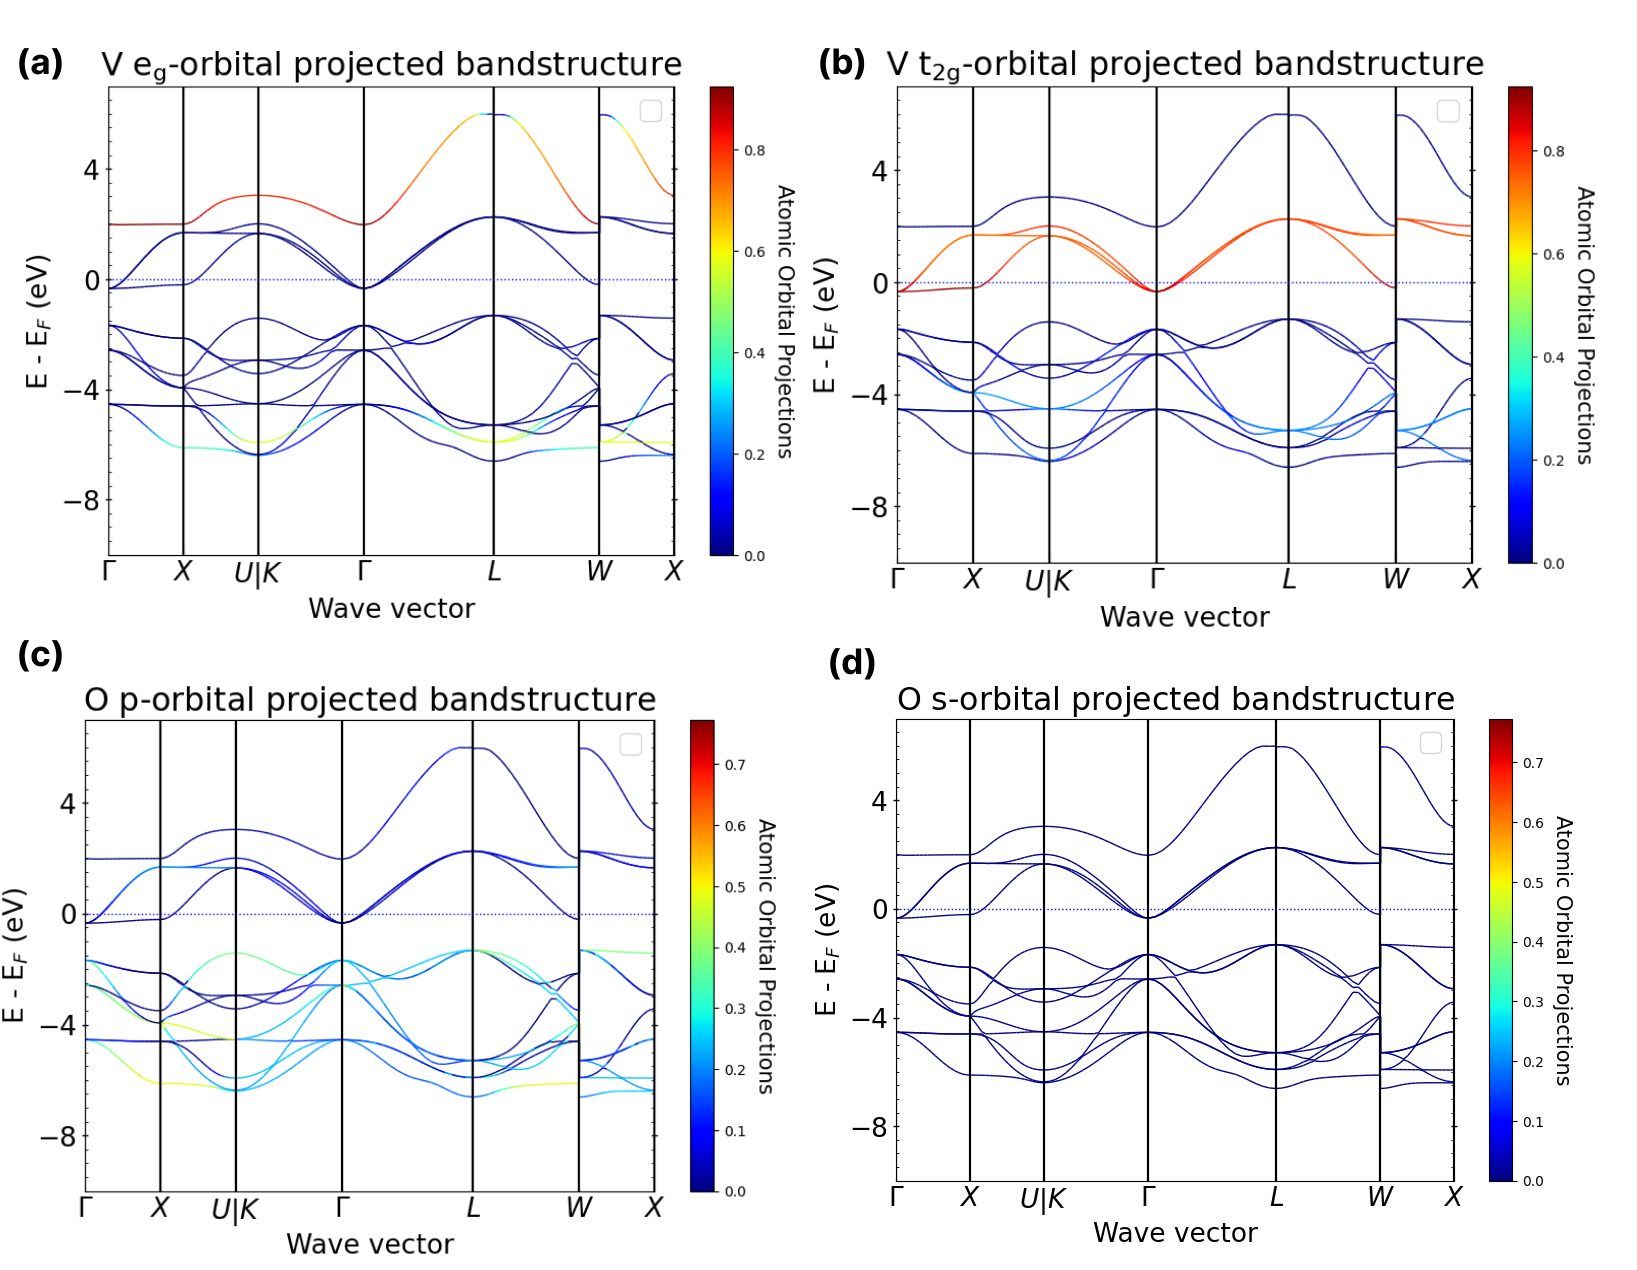
\includegraphics[width=\linewidth]{figs/BandStructure_SrVO3.png}
    \caption{
Projected band structure of \ch{SrVO3}, illustrating the separation between \(t_{2g}\) and \(e_g\) states for the vanadium \(d\)-orbitals and the oxygen \(p\)-orbitals. Panel (a) V \(t_{2g}\)-orbital projected band structure, (b) V \(e_g\)-orbital projected band structure, (c) O \(p\)-orbital projected band structure, (d) O \(s\)-orbital projection. From Panel (d), we observe that none of the band in the displayed energy range has a predominant O\(s\)-orbital character. The Fermi Energy is found to be \(4.7546 \, \text{eV}\), and the energy bands are plotted with respect to it. }
\label{fig:SrVO3-bandstructure}
\end{figure}
\begin{table}[H]
\centering
\caption{Crystal field splitting values for different bands included in the Wannier construction, with associated errors.}
\begin{tabular}{|l|c|c|c|}
\hline
\textbf{Bands used in} & \textbf{Symbol} & \textbf{Value [eV]} & \textbf{Error [eV]} \\ 
\textbf{WFs} & & & \\ \hline
only V-\(d\) & $\epsilon_{e_g}^{(d)} - \epsilon_{t_{2g}}^{(d)}$ & 2.8099 & 0.0003\\ \hline
V-\(d\) and O-\(p\) & $\epsilon_{e_g}^{(dp)} - \epsilon_{t_{2g}}^{(dp)}$ & 1.787616 & 0.001 \\ \hline
\end{tabular}
\label{table:splitting-SrVO3}
\end{table}
Finally, accuracy of our TB modelfor \ch{SrVO_3} is validated by verifying that the atomic positions align with the final Wannier centers. Moreover, the WFs interpolated bandstructure is calculated using both sets of Wannier functions. We note that both sets of Wannier functions perform equally well in reconstructing the band structure within the energy range of 2 to 5 eV, where the \(d\)-orbitals of V dominate the electronic states, as seen from Figure \ref{fig:SrVO3-reconstructed-bandstructure}.
We note that in the first set of Wannier functions, where MLWFs were constructed solely for the \(d\)-orbital bands, the interpolated band structure naturally reproduces only the \(d\)-band contributions. 
\subsection{\ch{PbTiO_3}}
Similarly, we examine \ch{PbTiO_3}, another cubic perovskite oxide, where Ti is in the \(3+\) oxidation state with a \(3d^1\) configuration. The band structure of \ch{PbTiO_3}, shown in Figure~\ref{fig:TiPbO3-bandstructure}, reveals significantly mixed orbital character compared to \ch{SrVO_3}. Unlike \ch{SrVO_3}, which exhibits distinct \(t_{2g}\) and \(e_g\) bands due to strong crystal field splitting and minimal hybridization, the bands in \ch{PbTiO_3} overlap considerably, reflecting a higher degree of hybridization.
We follow a similar workflow as before. The first set of Wannier functions is constructed using 5 Ti-centered WFs, focusing on bands between \(7 \, \text{eV}\) and \(14 \, \text{eV}\) relative to the Fermi energy. For the second set, the energy range is expanded to \(-1.8 \, \text{eV}\) to \(14 \, \text{eV}\) to include \(p\)-orbital-centered Wannier functions, adding 9 WFs corresponding to the three oxygen atoms in the unit cell. Finally, the energy range is extended further to \(-11.6 \, \text{eV}\) to \(14 \, \text{eV}\), incorporating \(s\)-orbital-centered Wannier functions for oxygen and resulting in a total of 17 WFs in the third set.
As shown in Table~\ref{table:splitting-TiPbO3}, the crystal field splitting decreases with the inclusion of oxygen \(p\)- and \(s\)-orbital-centered WFs, similar to the trend observed in \ch{SrVO_3}. This reduction highlights the impact of hybridization on the crystal field splitting, as seen in the first set of WFs, which reconstructs the \(d\)-orbital bands separately. Moreover, the smaller set of WFs again results in larger spreads, as seen by comparing Table \ref{table:wannier-centers-TiPbO3} with Table \ref{table:wannier-centers-TiPbO3-1}. However, we verify that, for all three sets, the first WFs have Cartesian coordinates matching those of the titanium ions, as expected. The interpolated band structure for all three sets of WFs is reported in Figure~\ref{fig:TiPbO3-reconstructed-bandstructure} in the Appendix.
\begin{figure}[htp]
    \centering
    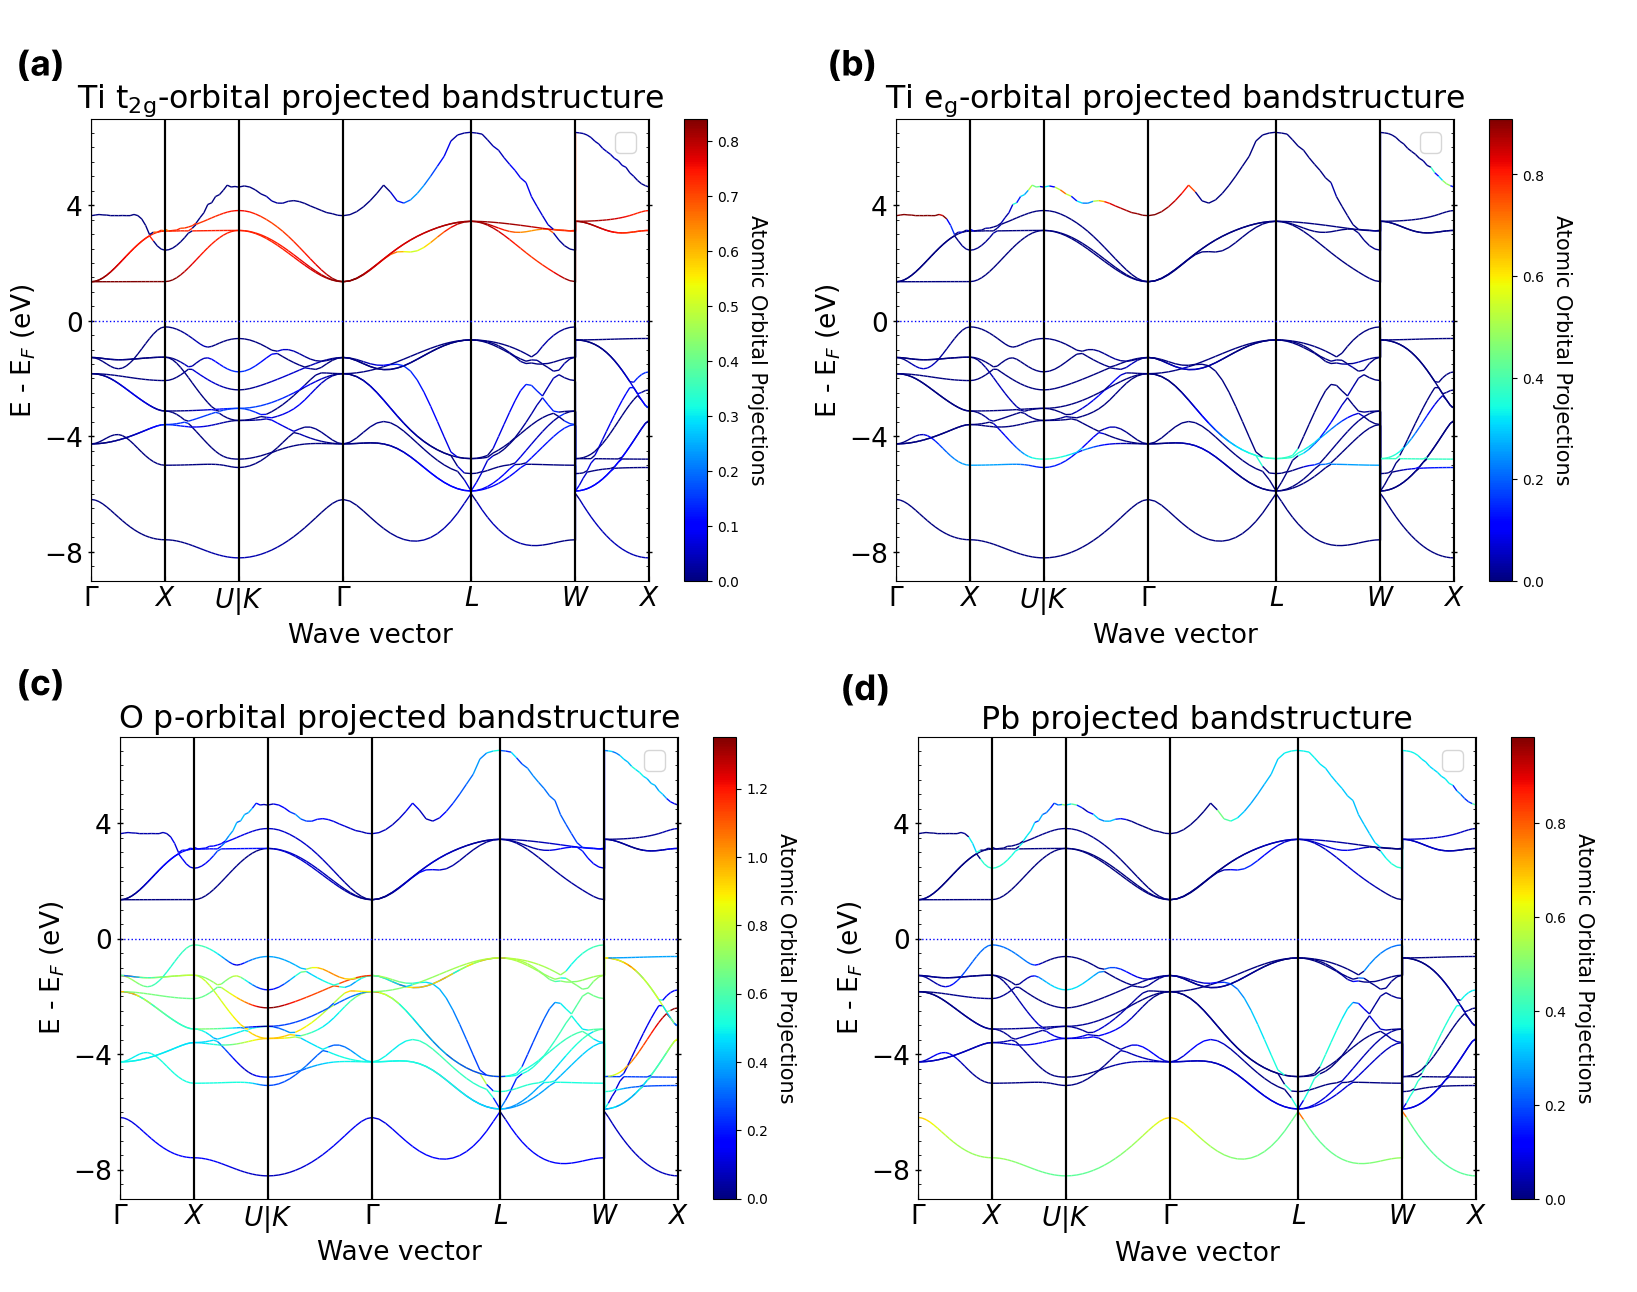
\includegraphics[width=\linewidth]{figs/BandStructure_TiPbO3.png}
\caption{
Projected band structure of \(\text{TiPbO}_3\) illustrating the orbital character contributions from different atomic species. (a) Ti \(t_{2g}\)-orbital projected band structure, (b) Ti \(e_g\)-orbital projected band structure, (c) O \(p\)-orbital projected band structure, and (d) Pb projected band structure. Unlike in \(\text{SrVO}_3\), the bands in \(\text{TiPbO}_3\) show significant orbital mixing, with no clear separation between the \(t_{2g}\) and \(e_g\) states. The Fermi Energy was found to be \(6.17 \, \text{eV}\), and the energy bands are plotted with respect to it. }
\label{fig:TiPbO3-bandstructure}
\end{figure}





\begin{table}[H]
\centering
\caption{Crystal field splitting values for different bands included in the Wannier construction, with associated errors}
\begin{tabular}{|l|c|c|c|}
\hline
\textbf{Bands used in} & \textbf{Symbol} & \textbf{Value [eV]} & \textbf{Error [eV]} \\ 
\textbf{WFs constr} & & & \\ \hline
only V-\(d\) & $\epsilon_{e_g}^{(d)} - \epsilon_{t_{2g}}^{(d)}$ & 2.230 & 0.003\\ \hline
V-\(d\) and O-\(p\) & $\epsilon_{e_g}^{(dp)} - \epsilon_{t_{2g}}^{(dp)}$ & 0.913 & 0.003 \ \\ \hline
V-\(d\), O-\(p\), and O-\(s\) & $\epsilon_{e_g}^{(dps)} - \epsilon_{t_{2g}}^{(dps)}$ &  0.890  &0.001 \\ \hline
\end{tabular}
\label{table:splitting-TiPbO3}
\end{table}
The lack of clear separation among the Ti \(t_{2g}\), Ti \(e_g\), and O \(p\) bands in the band structure of \ch{TiPbO_3} is an indication of the greater degree of hybridization between the Ti \(d\)-orbitals and the oxygen \(p\)-orbitals in this system. This is further confirmed by the larger difference in crystal field splitting (more than \(1, \, \text{eV}\) as it was for \ch{SrVO_3}) obtained from the two distinct sets of Wannier functions: one constructed using only the bands with \(3d\)-orbital character and the other including oxygen orbitals. 


\section{METHODS}
\subsection*{Density functional theory calculations} 
 The calculations for the electronic structure of \ch{SrVO_3} and \ch{TiPbO3} have been carried out using DFT with the Projector Augmented Wave (PAW) method \cite{ProjectorAugmentedWaveMethod}, as implemented in the Vienna ab initio Simulation Package ~\cite{Kresse1993, Kresse1994, Kresse1996Efficiency, Kresse1996Efficient} (VASP) version 5.4.4.
 The VASP-supplied PBE~\cite{PBE1996} PAW potentials version 5.4 were used, with the value of the valency of each atomic sphere being 10 for strontium, 5 for vanadium, 6 for oxygen, and 14 for both titanium and lead. 
 A plane wave kinetic energy cutoff of 550 eV was used, together with an electronic convergence threshold of 10$^{-6}$ eV and a threshold of maximum force of any one ion of 10$^{-2}$ eV {\AA}$^{-1}$. The NSW parameter in VASP allowed for a maximum of 50 ionic steps for the system to relax into its ground state.
 The Brillouin zone was sampled using a Monkhorst-Pack mesh with a spacing of 0.02 {\AA}$^{-1}$, and the width of the Gaussian smearing set to 0.01 eV.
In all calculations, we employ non-spin-polarized DFT, as this approach is consistent with the fact that both \ch{SrVO_3} and \ch{PbTiO_3} are non-magnetic systems.

\subsection*{Point-charge model (PCM)}
The classical point charge model is a classical approach used to estimate the crystal field splitting in transition metal complexes and solid-state systems. This model represents the simplest form of the crystal field, where the lattice is replaced by an array of point charges located at the nuclei of the constituent ions \cite{Morrison1988}, and the crystal field splitting parameter \(\Delta_{\text{o}}\) is estimated by considering the electrostatic interaction between a central metal ion and surrounding ligands \cite{Bethe1929}.
For an octahedral arrangement, the potential \(V(r, \theta, \phi)\) at the metal ion due to ligands can be expanded in spherical harmonics. The dominant term for crystal field splitting is \(V_{40}\), which is proportional to \(\sum_i \frac{q_i}{a^5}\), where \(q_i\) are the ligand charges and \(a\) is the metal-ligand distance. This yields the following crystal field splitting equation:

\begin{equation}
    \Delta_{\text{o}} = \frac{5Ze^2}{12\pi\varepsilon_0 a^5} \langle r^4 \rangle = \frac{5k}{3} \frac{Ze^2}{a^5} \langle r^4 \rangle,
\label{eq:CFT_10Dq}
\end{equation}

where \(Z\) is the effective nuclear charge of the ligand (\(Z=2\) for \(\ch{O^{2-}}\), \(e\) is the elementary charge, \(\varepsilon_0\) is the permittivity of free space, and \(\langle r^4 \rangle\) is the average of the fourth power of the \(nd^3\)-electron radial coordinate in the transition metal, which for both \ch{V^{4+}} and \ch{Ti^{3+}} can be estimated to be \(0.173 \times 10^8 pm^4\) \cite{Rogers2014}. 

To extract \(\Delta_{\text{o}}\) using the PCM, we focused on a single \(\ch{VO_6}\) octahedral unit within the lattice of the relaxed structure of the conventional unit cell of \ch{SrVO_3} (or \ch{TiPbO_3} ), and looked at the metal (\(\ch{V^{4+}}\))-ligand (\(\ch{O^{2-}}\)) distances. The metal-ligand distance in \ch{SrVO_3} is \(a_V = 1.90813 \, \text{\AA}\) and \(a_{Ti} = 1.96092 \, \text{\AA}\) in  \ch{TiPbO_3}. Using Equation \ref{eq:CFT_10Dq}, we derived a  \(\Delta_{\text{o}}\) of \(2.6110  \, \text{eV}\) and \(2.2785 \, \text{eV}\) for \(\text{SrVO}_3\), and \(\text{TiPbO}_3\), respectively


\section{Summary \& Conclusion}
Using the combined capabilities of DFT and the MLWF formalism, we have investigated the crystal field splitting \(\Delta_{\text{o}}\) for \(\ch{V^{4+}}\) in the octahedral environment of \(\ch{VO_6}\) in \ch{SrVO3}, and for \(\ch{Ti^{3+}}\) of  \(\ch{TiO_6}\) in \ch{PbTiO3}. The crystal field splitting was determined by evaluating the on-site energies of the \(d\)-orbitals from a tight-binding (TB) model constructed with Maximally Localized Wannier Functions (MLWFs), which were designed to closely resemble the atomic \(d\)-orbitals of \(\ch{V^{4+}}\) (or \(\ch{Ti^{3+}}\)). 
First, for  \ch{SrVO3},  by constructing a tight binding model using Wannier functions projected solely onto the \(d\)-orbitals, we found the crystal field splitting to be \(2.81 \, \text{eV}\). When Wannier functions centered on the \(p\)-orbitals of oxygen were also included, the Wannier functions became more localized, resulting in a reduced crystal field splitting of \(1.79 \, \text{eV}\).  This decrease in crystal field splitting demonstrates the sizeable contribution from hybridization with surrounding ligand \(p\)-orbitals to the ligand field, highlighting the importance of including these interactions in accurate modeling of crystal field effects. 
This analysis also allowed us to conclude that for \ch{SrVO3}, the total \(e_g\)-\(t_{2g}\) splitting of \(2.69 \, \text{eV}\) comprises contributions from different sources. To isolate the pure electrostatic contribution to the crystal field splitting, one would need to compute a set of Wannier functions centered on all orbitals. Based on the two sets of Wannier functions constructed in this study, we estimate that approximately \(2.81 - 1.79 = 1.02 \, \text{eV}\) arises from \(d\)-\(p\) hybridization. However, since the \(1.79 \, \text{eV}\) value also likely includes contributions from \(d\)-\(p\) hybridization, a even more comprehensive Wannier function construction would be needed to fully disentangle the various contributions to the crystal field splitting.
The tight binding construction for  \ch{TiPbO3} turned out to be more difficult; none of the three sets of WFs yielded a interpolated bandstructure that perfectly resembled the DFT-computed bandstructure, as we were able to derive for \ch{SrVO_3}
As a final step, we compared the above result obtained using Wannier functions with the prediction from the classical point charge model (see Methods section for details). Using this model, we derive a crystal field splitting value of \(2.611  \, \text{eV}\) and \(2.2785 \, \text{eV}\) for \ch{SrVO_3}, and \ch{TiPbO_3}, respectively. In both cases, the classical point charge model overestimates the crystal field splitting compared to the results obtained using Wannier functions. 
\begin{acknowledgments}
I acknowledge the computation time provided by the Quantum Matter Institute's computing cluster, as well as Professor Joerg Rottler at the University of British Columbia for granting access to the VASP license.
\end{acknowledgments}

\appendix

\section{}
\begin{table}[H]
\centering
\begin{tabular}{|l|c|c|}
\hline
 & \textbf{Only V-\(d\)} & \textbf{V-\(d\) + O-\(p\)} \\ \hline
$\epsilon_{d_{xy}}$ &  6.060837 &  4.895412 \\ \hline
$\epsilon_{d_{yz}}$ & 6.060826 & 4.895382 \\ \hline
$\epsilon_{d_{zx}}$ &  6.060827 & 4.895382 \\ \hline
\textbf{Mean ($ \varepsilon_{t_{2g}}$)} & \(6.06083 \pm 0.00001 \) & \(4.895392 \pm 0.00001 \) \\ \hline
$\epsilon_{d_{x^2-y^2}}$ & 8.87040  & 6.681992 \\ \hline
$\epsilon_{d_{z^2}}$ & 8.87040  & 6.684025\\ \hline
\textbf{Mean ($ \varepsilon_{e_{g}}$)} & $8.8707115  \pm  0.0003$  &\(6.6830085 \pm 0.001 \) \\ \hline
\end{tabular}
\label{table:SrVO3-onsite-energies}
\caption{Comparison of on-site energies and crystal field splitting values for \ch{V^{4+}}-centered \(d\)-like Wannier functions constructed using only \(3d\) orbitals versus including both \(3d\) and oxygen \(p\) orbitals. The uncertainties for the \(t_{2g}\) and \(e_g\) mean values were calculated based on the standard deviation divided by the square root of the sample size (3 for \(t_{2g}\) and 2 for \(e_g\)). Note: for the 2nd set, we are omitting the on-site energies of the 9 WFs centered on the p-orbitals of oxygen, as we are only interested in reporting the on-site energies of the \ch{V^{4+}}-centered \(d\)-like Wannier functions.}
\end{table}

\begin{table}[H]
\centering

\begin{tabular}{|c|c|c|}
\hline
\textbf{WF Number} & \textbf{Center Coordinates (Å)} & \textbf{Spread (Å\(^2\))} \\ \hline
1 & (1.908129, 1.908129, 1.908129) & 3.29851247 \\ \hline
2 & (1.908129, 1.908129, 1.908129) & 1.95264099 \\ \hline
3 & (1.908129, 1.908129, 1.908129) & 1.95265841 \\ \hline
4 & (1.908129, 1.908129, 1.908129) & 3.40400305 \\ \hline
5 & (1.908129, 1.908129, 1.908129) & 1.95267656 \\ \hline
\end{tabular}
 \label{table:wannier-centers-SrVO3}
 \caption{WF centers and spreads for vanadium-centered Wannier functions in SrVO\(_3\), when we only include the d-orbitals of vanadium in the construction of the tight binding model.}
\end{table}

\begin{table}[H]
\centering

\begin{tabular}{|c|c|c|}
\hline
\textbf{WF Number} & \textbf{Center Coordinates (Å)} & \textbf{Spread (Å)} \\ \hline
1 & (1.908067, 1.908129, 1.906649) & 1.27536288 \\ \hline
2 & (1.908134, 1.908129, 1.908135) & 0.75179643 \\ \hline
3 & (1.908129, 1.908129, 1.908142) & 0.75175883 \\ \hline
4 & (1.907745, 1.908130, 1.908096) & 1.31876994 \\ \hline
5 & (1.908141, 1.908129, 1.908129) & 0.75175691 \\ \hline
\end{tabular}
\caption{WF centers and spreads for vanadium-centered Wannier functions in SrVO\(_3\) when we include both the  oxygen p orbitals in the construction of the tight-binding model.}
 \label{table:wannier-centers-SrVO3-2}
\end{table}

\begin{figure}[H]
    \centering
    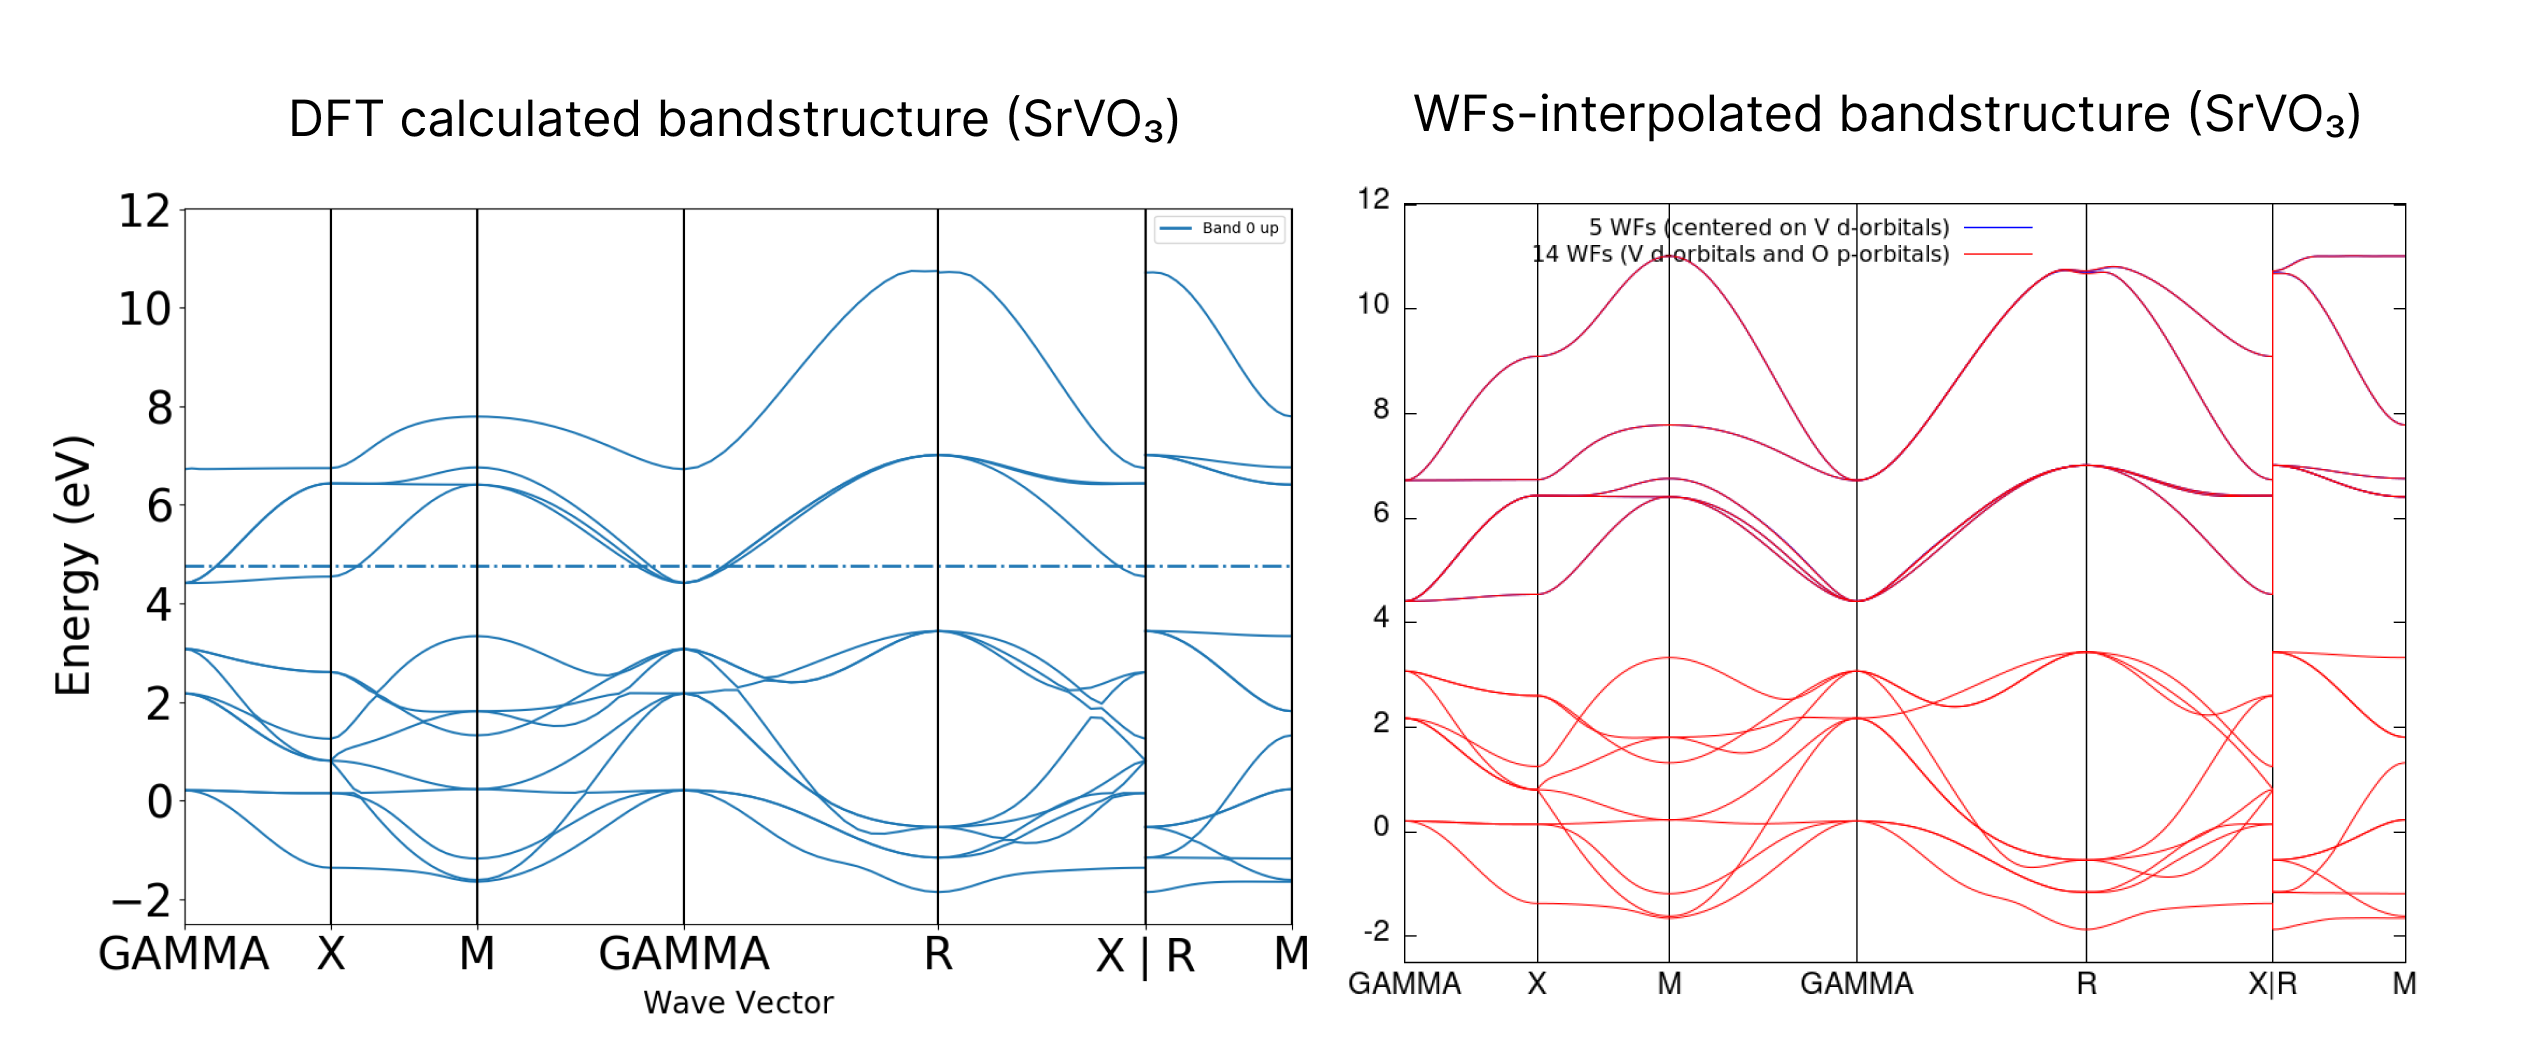
\includegraphics[width=\linewidth]{figs/comparison_SrVO3.png}
   \caption{
Comparison of DFT computed bandstructure and reconstructed band structure of \ch{SrVO3} using two different sets of Wannier functions (WFs). The blue lines represent the band structure reconstructed with 5 WFs centered on the V \(d\)-orbitals, while the red lines represent the reconstruction with 14 WFs, including both V \(d\)-orbitals and O \(p\)-orbitals. Although the inclusion of O \(p\)-orbitals in the Wannier construction (14 WFs) leads to a more accurate representation of the full electronic structure, the quality of the Wannier-interpolated band structure is very similar. 
}
\label{fig:SrVO3-reconstructed-bandstructure}
\end{figure}

\begin{table}[H]
\centering
\begin{tabular}{|l|c|c|}
\hline
\textbf{Quantity} & \textbf{Only Ti-\(d\)} & \textbf{Ti-\(d\) + O-\(p\)} \\ \hline
$\epsilon_{d_{xy}}$ & 9.589241 & 8.31594 \\ \hline
$\epsilon_{d_{yz}}$ & 9.58921 & 8.315581 \\ \hline
$\epsilon_{d_{zx}}$ & 9.583362 & 8.309073 \\ \hline
\textbf{Mean ($E_{t_{2g}}$)} & \(9.587271 \pm 0.003 \) & \( 8.313531333 \pm 0.003 \)\\ \hline
$\epsilon_{d_{x^2-y^2}}$ & 11.899884 & 9.406448 \\ \hline
$\epsilon_{d_{z^2}}$ & 11.73462 & 9.04755  \\ \hline
\textbf{Mean ($E_{e_{g}}$)} & \(11.817252\pm 0.08 \) & \(9.226999 \pm 0.2 \)  \\ \hline
\textbf{$\Delta_{\text{o}}$} & \(2.229981 \pm 0.001 \) &  0.913467667 \\ \hline
\end{tabular}
\caption{Comparison of on-site energies and crystal field splitting values for \ch{Ti^{3+}}-centered \(d\)-like Wannier functions constructed using only \(3d\) orbitals versus including both \(3d\) and oxygen \(p\) orbitals. Averages, associated uncertainties, and crystal field splitting values are shown.}
\end{table}

\begin{table}[H]
\centering

\begin{tabular}{|c|c|c|}
\hline
\textbf{WF Number} & \textbf{Center Coordinates (Å)} & \textbf{Spread (Å\(^2\))} \\ \hline
1 & (1.990002, 1.965455, 1.963597) & 15.56094260 \\ \hline
2 & (1.960919, 1.960949, 1.960905) & 1.67887288 \\ \hline
3 & (1.960903, 1.960921, 1.960912) & 1.68398896 \\ \hline
4 & (1.941535, 1.952037, 1.965810) & 18.87839696 \\ \hline
5 & (1.960920, 1.960955, 1.960918) & 1.67569860 \\ \hline
\end{tabular}
\caption{WF centers and spreads for vanadium-centered Wannier functions in \ch{TiPbO_3}, when we only include the d-orbitals of titanium in the construction of the tight binding model.}
\label{table:wannier-centers-TiPbO3}
\end{table}

\begin{table}[H]
\centering
\begin{tabular}{|c|c|c|}
\hline
\textbf{WF Number} & \textbf{Center Coordinates (Å)} & \textbf{Spread (Å\(^2\))} \\ \hline
1 & (2.043523, 2.051313, 2.088552) & 8.20037992 \\ \hline
2 & (1.960849, 1.961052, 1.960702) & 0.78445781 \\ \hline
3 & (1.960981, 1.961029, 1.960914) & 0.78540027 \\ \hline
4 & (1.939829, 1.947476, 2.053274) & 8.27652261 \\ \hline
5 & (1.960853, 1.960899, 1.961115) & 0.79083593 \\ \hline
\end{tabular}
\label{table:wannier-centers-TiPbO3-1}
\caption{WF centers and spreads for titanium-centered Wannier functions in \ch{TiPbO_3} when we include the d-orbitals of titanium and the oxygen p orbitals in the construction of the tight-binding model.}
\end{table}

\begin{figure}[H]
    \centering
    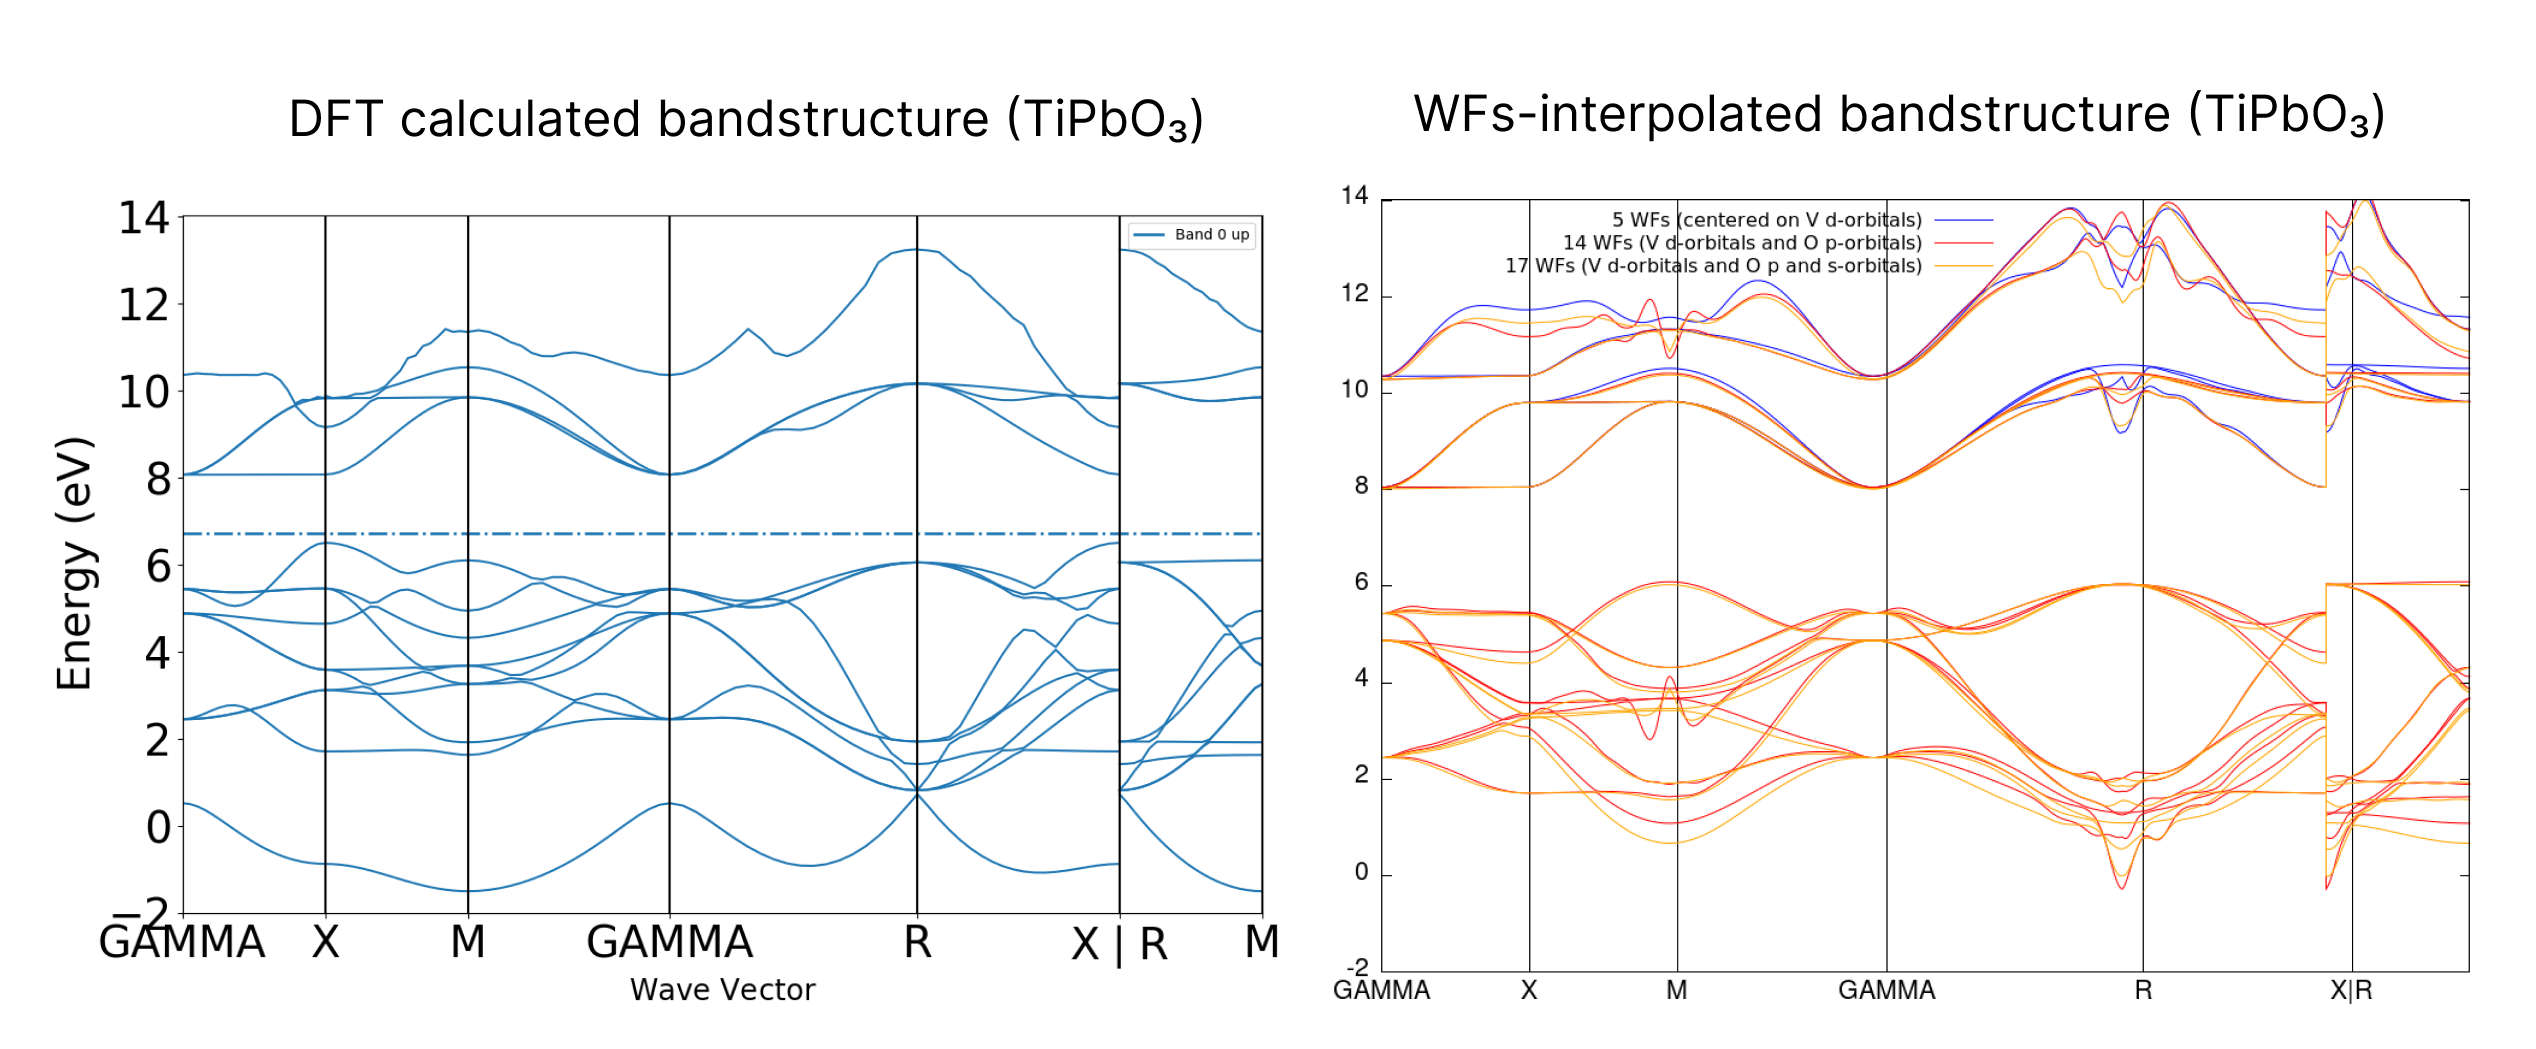
\includegraphics[width=\linewidth]{figs/comparison_TiPbO3.png}
   \caption{
Comparison of DFT computed bandstructure and reconstructed band structure of \ch{TiPbO3} using three different sets of Wannier functions (WFs). The blue lines represent the band structure reconstructed with 5 WFs centered on the Ti \(d\)-orbitals, while the red lines represent the reconstruction with 14 WFs, including both Ti \(d\)-orbitals and O \(p\)-orbitals. The orange line represents the interpolated band structure using 17 WFs, including both Ti \(d\)-orbitals and O \(p\)-orbitals. . 
}
\label{fig:TiPbO3-reconstructed-bandstructure}
\end{figure}
% The \nocite command causes all entries in a bibliography to be printed out
% whether or not they are actually referenced in the text. This is appropriate
% for the sample file to show the different styles of references, but authors
% most likely will not want to use it.
\nocite{*}

\bibliography{apssamp}% Produces the bibliography via BibTeX.

\end{document}
%
% ****** End of file apssamp.tex ******
